\chapter{Inverted Pendulum Analysis}


\section{Inverted Pendulum Description}\label{sec:IPDesc}
For this project an inverted pendulum set up is given. It consists of:
\begin{itemize}
	\item A DC motor
	\item A gear system
	\item An arm
	\item A stick connected to the end of the arm.
\end{itemize}
A diagram of the setup when fully assembled is seen on \autoref{fig:InvertedPendulumSetUp}.

\begin{figure} [htbp]
	\centering
	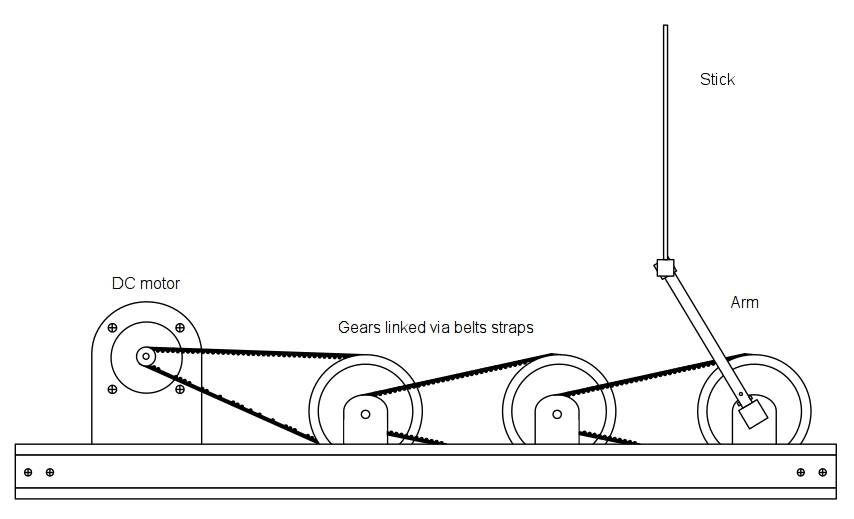
\includegraphics[width=0.6\linewidth]{figures/"Preanalysis&Requirement"/invertedPendulumDiagram}
	\caption{Diagram of the set up fully assembled.} \label{fig:InvertedPendulumSetUp}
\end{figure}

\section{Inverted Pendulum Hardware}
The following section describes the hardware connected to the inverted pendulum setup illustrated cf. figure \ref{fig:InvertedPendulumSetUp}.
Each part will be described with its specifications and use in the setup.

\subsubsection{Stick and Arm}
The arm and stick is elements that always appears in the double inverted pendulum setup. The goal is for the arm to apply force on the joint, which would affect the position of the stick. 

Stick length: 80 cm
Stick weight: 344 grams

Stick length: 40 cm
Stick weight: 170 grams
 
Arm length: 33 cm
Arm weight: 288 grams

\subsubsection{DC Motor}
Alsthom BBC MODEL: F9M2 AAU:08339
\ref{appendix:DCMotorInductance}

\subsubsection{Gear System}
Gear teeth big: 40
Gear teeth small: 12
Belt length: 60 cm
Wheel diameter big: 12 cm
Wheel diameter small: 4 cm


\section{Modelling of the Arm and Stick}\label{sec:StickArm}

%%%%%%%%%%%%% Equation template %%%%%%%%%%%%%%%
%\begin{flalign}
%\hspace{30pt} & EQUATION1 &&& \text{[UNIT]} \notag \\
%& EQUATION2 &&& \text{[UNIT]} \label{eq:LABEL} 
%\end{flalign}
%\begin{description}
%  \item[\hspace{30pt}\textnormal{where:}]\hfill \\
%  \begin{tabular}{p{30pt}lp{250pt}l}
%& $x$ & TEXT & [UNIT]  \\
%& $y$ & VERY LONG TEXT THAT IS VERY LONG AND HAS A LOT OF WORDS IN IT YET THE FORMATTING STILL LOOKS NICE AND CLEAN AND EVERYTHING IS AWESOME & [UNIT]  \\
%& $z$ & TEXT & [UNIT]
%\end{tabular}
%\end{description}
%%%%%%%%%%%%%%%%%%%%%%%%%%%%%%%%%%%%%%%%%%%%%%%
\graphicspath{{figures/modeling/ArmStick/}}
The goal of this section is to have a mathematical model for the behaviour of the angle of the stick in relation to the angle of the arm on the motor. The inputs and outputs of this system can be seen by the block diagram in \autoref{fig:StickBlock}.
\begin{figure}[htbp]
\centering
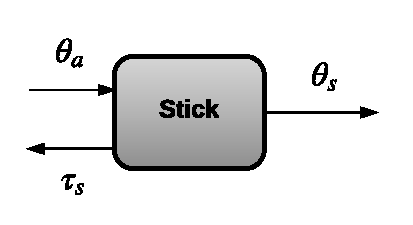
\includegraphics[width=0.4\textwidth]{InputOutputStick.pdf}
\caption{Block diagram of the inputs and outputs of the stick section of the inverted pendulum setup.}
\label{fig:StickBlock}
\end{figure}

The angles, constants and forces used to describe the system are seen on \autoref{fig:ArmStick}.
%\todo[inline,author=Jacob]{I'd like to somehow describe the process first instead of just going along randomly and suddenly ending up with the model. "We want to achieve this so we do that" etc.}
\begin{figure}[htbp]
\centering
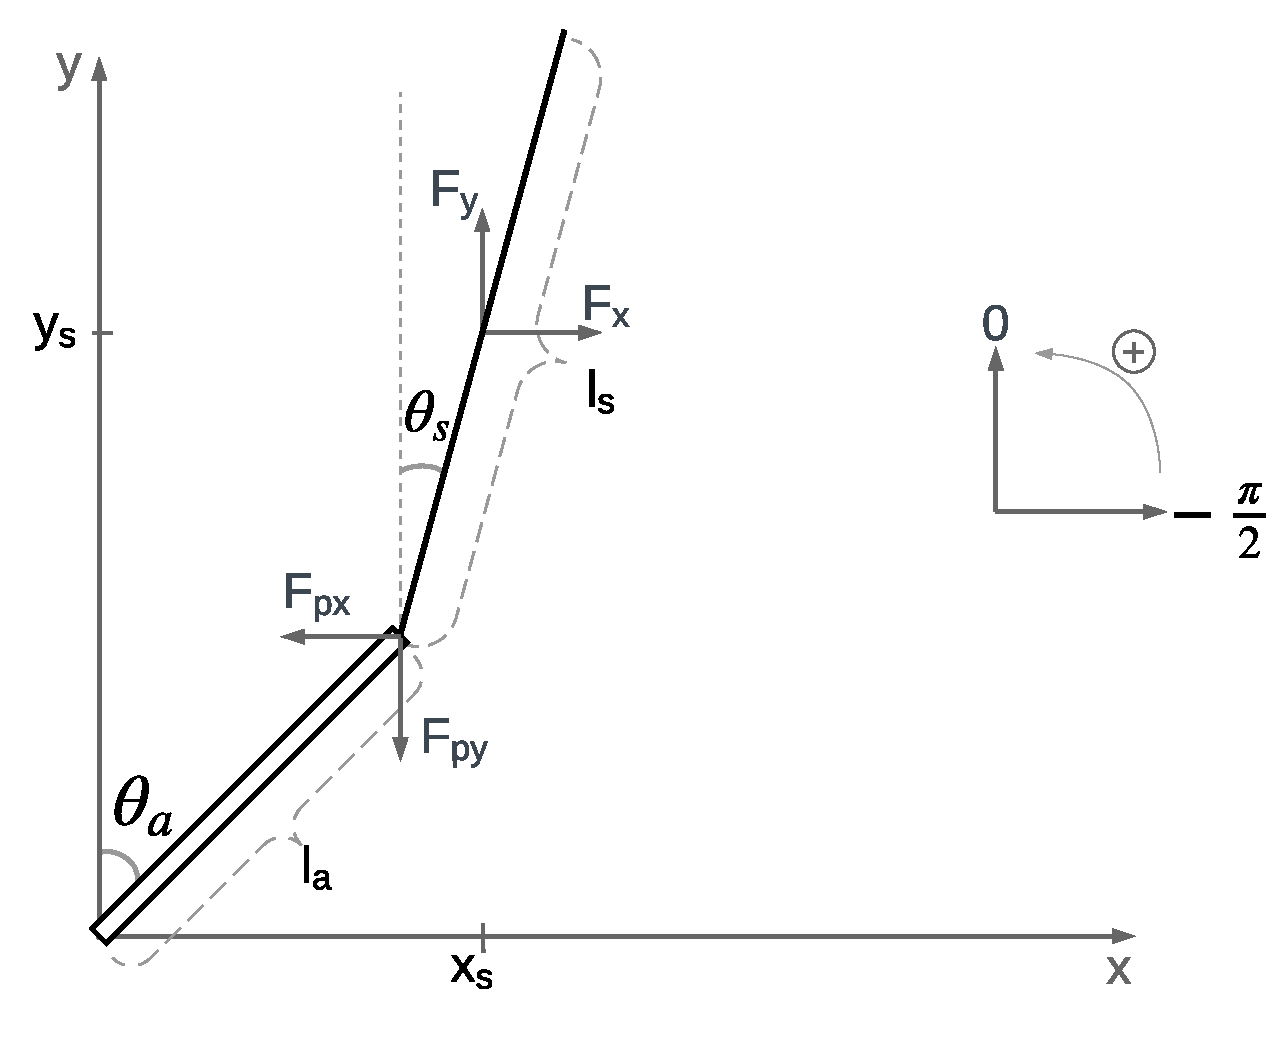
\includegraphics[width=0.8\textwidth]{StickAndForces}
\caption{Diagram of the angles and forces acting on the arm and the stick.}
\label{fig:ArmStick}
\end{figure}
\startexplain
	\explain{$F_x$ is the force in the x direction}{\si{\newton}}
	\explain{$F_y$ is the force in the y direction}{\si{\newton}}
	\explain{$x_s$ is the position of the center of mass of the stick in the x direction}{\si{\meter}}
	\explain{$y_s$ is the position of the center of mass of the stick in the y direction}{\si{\meter}}
	\explain{$l_a$ is the length of the arm}{\si{\meter}}
	\explain{$l_s$ is the length of the stick}{\si{\meter}}
	\explain{$\theta_a$ is the angle from the arm to the y-axis}{\si{\radian}}
	\explain{$\theta_s$ is the angle from the stick to the y-axis}{\si{\radian}}
\stopexplain
\todo[inline,author=Jacob]{Add the reactionary forces where arm and stick connects. Fpx and Fpy.}
All forces, constants and variables that relates to the arm and stick are denoted by a subscripted $a$ and $s$ respectively. 

The behaviour of the stick can be fully described by three movements; two translatory and one rotary. It can move in the x and y direction and rotate around it's own axis. To fully describe the system two geometric equations are also needed.

%To find the relation between the angles, the free body diagram of the joint of the arm and stick is made on \autoref{fig:freebodystick}.
%\begin{figure}[htbp]
%\centering
%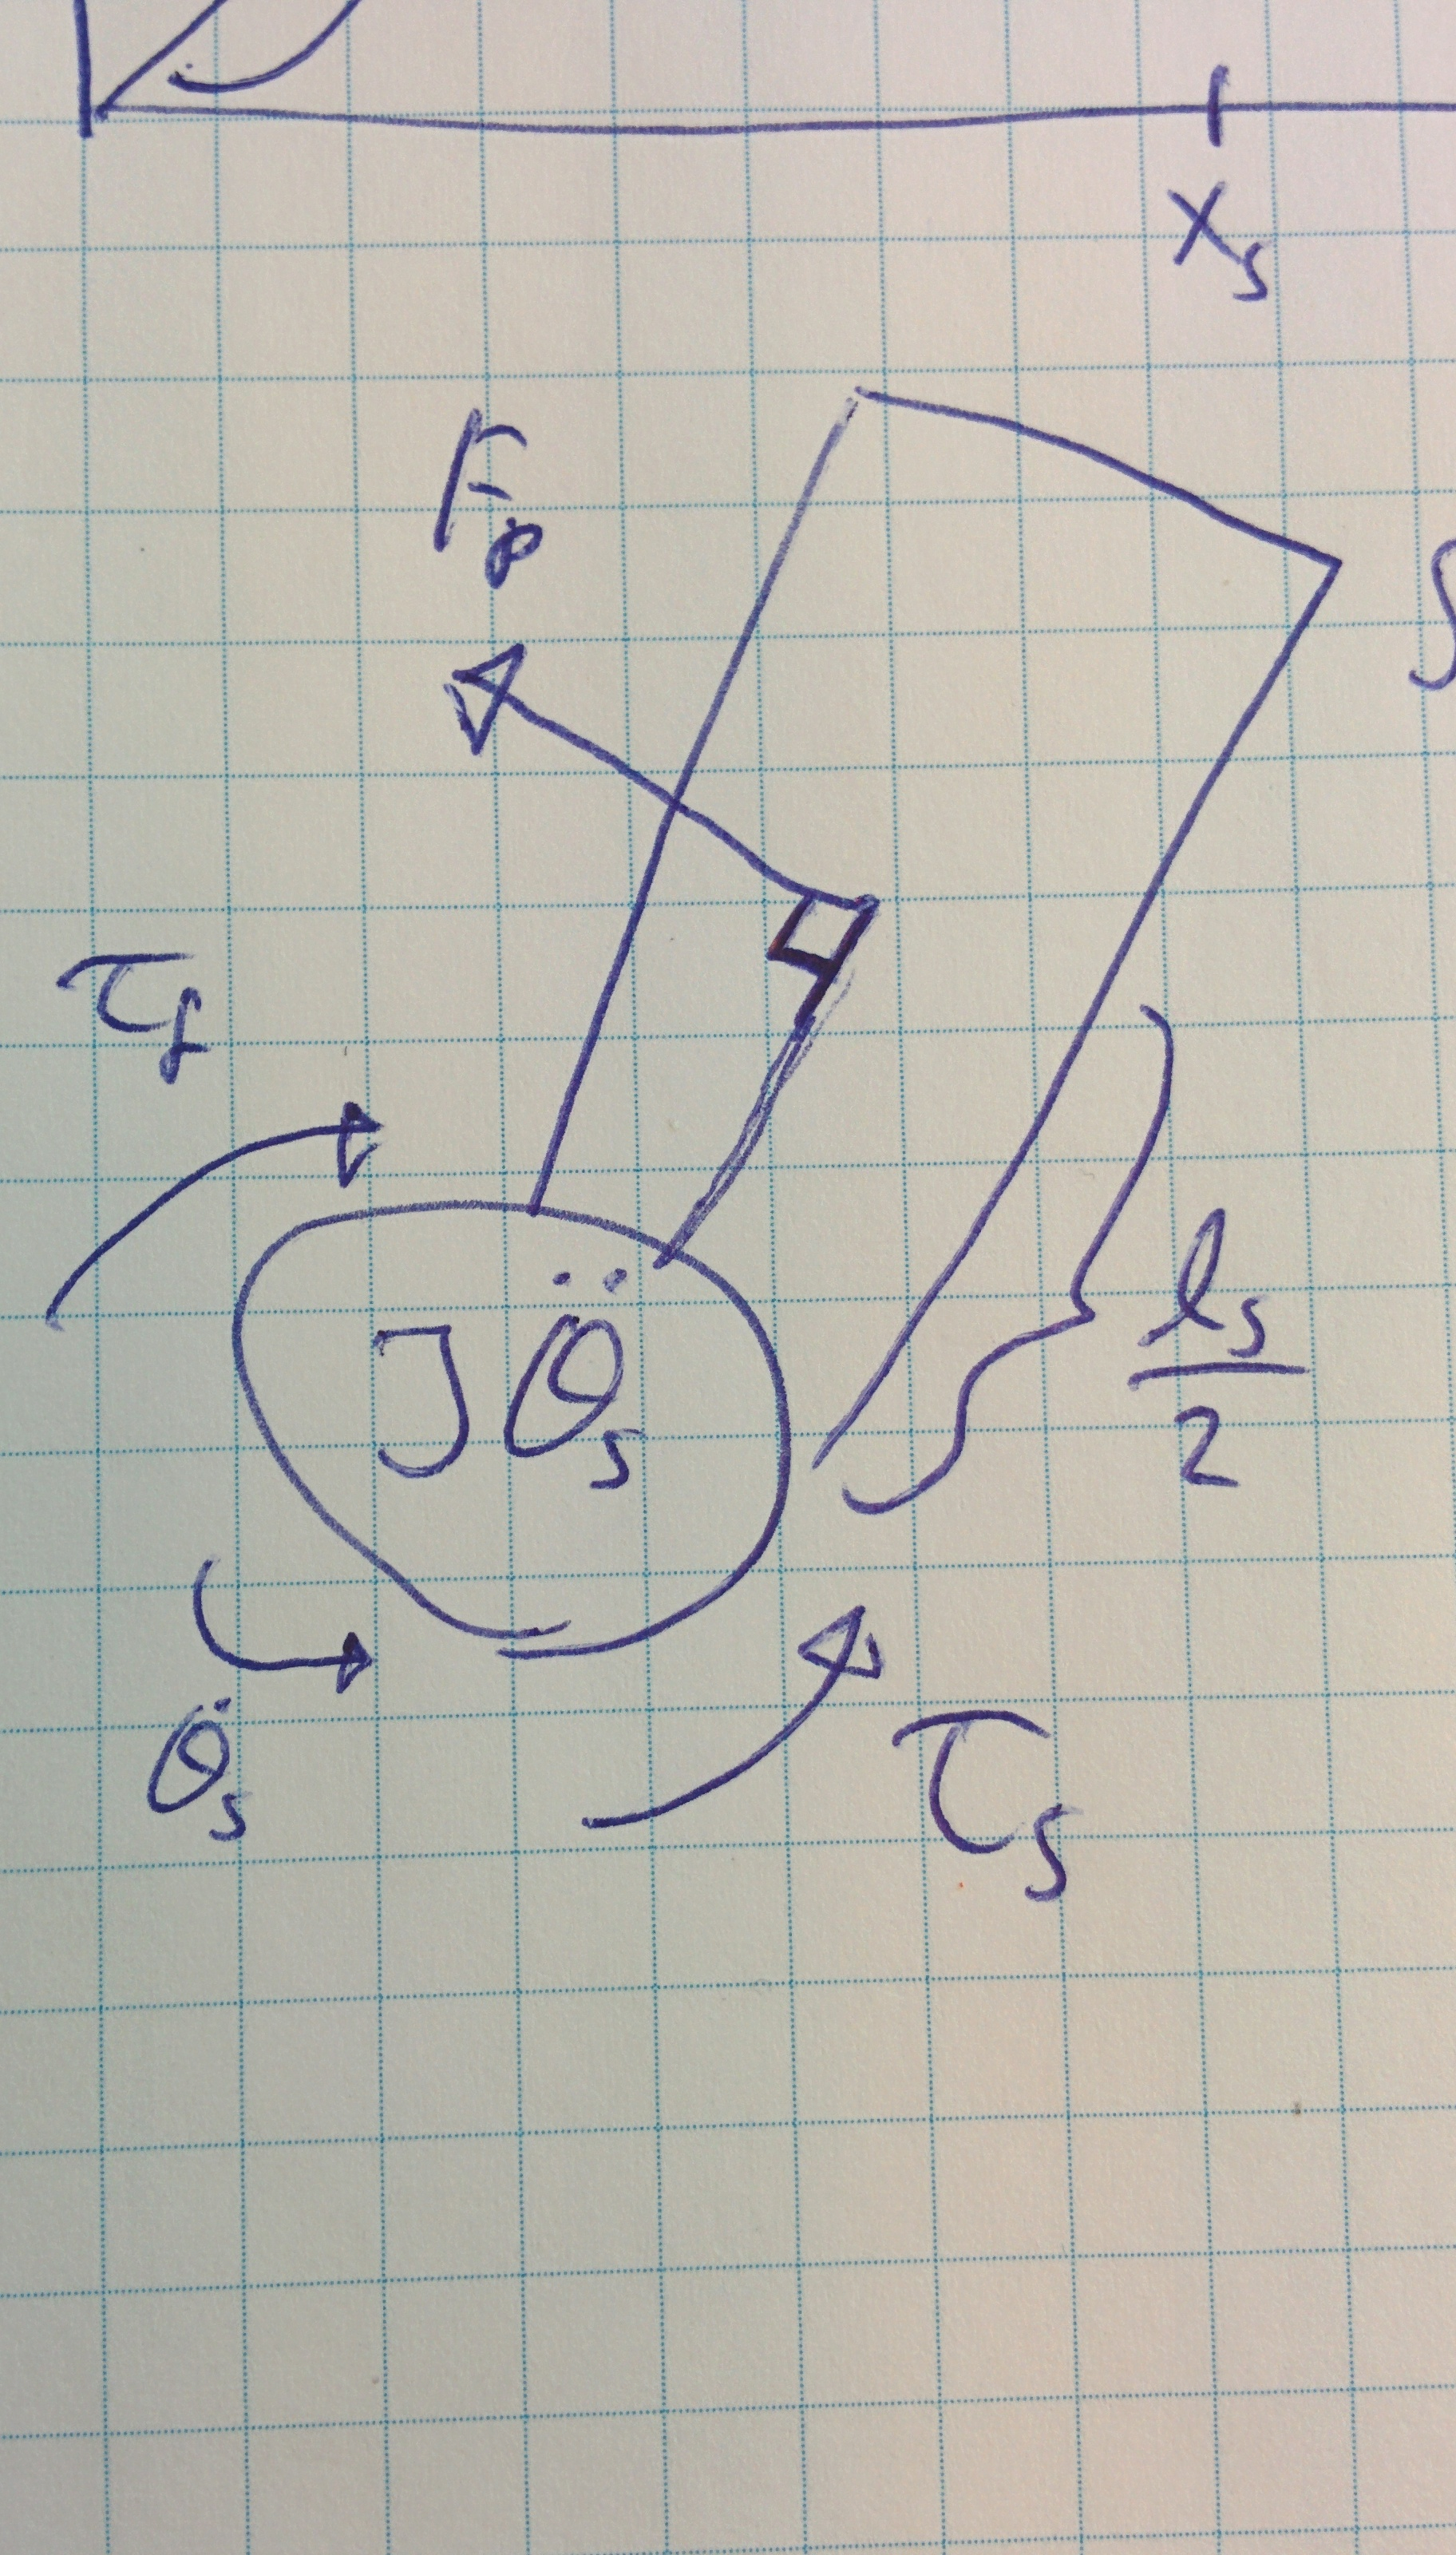
\includegraphics[width=0.25\textwidth]{FreeBodyPendulum}
%\caption{Free body diagram of the joint that connects the arm and the stick.}
%\label{fig:freebodystick}
%\end{figure}
%\todo[inline, author=Jacob]{Make pretty graph}
%
%The moment of inertia for the joint is described by \autoref{eq:Jsthetas}.
%\begin{subequations}
%\begin{flalign}
%& J_s\ddot{\theta}_s=\tau_s-\tau_f  \label{eq:Jsthetas} \\
%& \tau_s =F_p\frac{l_s}{2} \\
%& \tau_f =b_{as}\dot{\theta}_{as} 
%\end{flalign}
%\end{subequations}
%\startexplain
%	\explain{$J_s$ is the moment of inertia for the stick}{\si{\kg\square\meter}}
%	\explain{$\ddot{\theta}_s$ is the angular acceleration of the stick}{\si{\radian\per\square\second}}
%	\explain{$\tau_s$ is the torque induced by the rotation of the stick}{\si{\newton\meter}}
%	\explain{$\tau_f$ is the torque of the friction acting on the stick}{\si{\newton\meter}}
%	\explain{$F_p$ is the force perpendicular to the stick at the center of mass}{\si{\newton}}
%	\explain{$b_{as}$ is the viscous friction coefficient between the arm and the stick}{\si{\newton\meter\second}}
%	\explain{$\dot{\theta}_{as}$ is the difference in angular velocity between the arm and the stick ($\dot{\theta}_s-\dot{\theta}_a$)}{\si{\radian\per\second}}
%\stopexplain
%
%The friction is calculated from the difference in angular velocity as the stick could be perfectly upright while the arm moves causing the joint to turn. The angle of the arm is not considered as producing a torque acting on the joint but as part of the force on the stick, $F_p$.

The two translatory forces acting on the stick in the x and y directions are found by \autoref{eq:FxFy} using Newton's 2nd law of motion.
\begin{subequations}  \label{eq:FxFy}
\begin{flalign}
	& \ddot{x}_sM_s=F_x  \label{eq:transx} \\
	& \ddot{y}_sM_s=F_y-gM_s  \\
	& F_y=\left(\ddot{y}_s+g\right)M_s \label{eq:transy}
\end{flalign}
\end{subequations}
\startexplain
	\explain{$g$ is the standard gravitational acceleration near the surface of the earth}{\si{\meter\per\square\second}}
	\explain{$M_s$ is the mass of the stick}{\si{\kilo\gram}}
\stopexplain
The rotational movement of the stick is described by \autoref{eq:rotaryforce}.
\begin{flalign}
 J_s\ddot{\theta}_s &=\frac{l_s}{2}\left(F_x\cos(\theta_s)+F_y\sin(\theta_s)\right)-b_{as}\dot{\theta}_{as} \label{eq:rotaryforce}
\end{flalign}

Finally the position of the center of mass of the stick in the x and y direction is found by \autoref{eq:xsys} using geometry.
\begin{subequations}\label{eq:xsys} 
\begin{flalign}
& x_s=l_a\sin (-\theta_a)+\frac{l_s}{2} \sin (-\theta_s) \\
& x_s=-l_a\sin (\theta_a)-\frac{l_s}{2} \sin (\theta_s) \label{eq:geox} \\
& y_s = l_a\cos (-\theta_a)+\frac{l_s}{2} \cos(-\theta_s) \\
& y_s = l_a\cos (\theta_a)+\frac{l_s}{2} \cos(\theta_s) \label{eq:geoy}
\end{flalign}
\end{subequations}

\autoref{eq:transx}, \autoref{eq:transy}, \autoref{eq:rotaryforce}, \autoref{eq:geox} and \autoref{eq:geoy} are all the equations neccessary to fully describe the behaviour of the system. The goal of the modeling is to end with a transfer function that relates the angle of the stick to the angle of the arm. There are 6 unknown variables in the 5 equations: $F_x$, $F_y$, $x_s$, $y_s$, $\theta_a$ and $\theta_s$. It should therefore be possible to end with one equation with the two unknowns $\theta_a$ and $\theta_s$ i.e. the transfer function.

The derivatives of $x_s$ and $y_s$ is found in \autoref{eq:diffxy}.
\begin{subequations}\label{eq:diffxy} 
\begin{flalign}
\hspace{30pt} & \dot{x}_s=-l_a\dot{\theta}_a\cos(\theta_a)-\frac{l_s}{2}\dot{\theta}_s\cos(\theta_s) & [\si{\meter\per\second}] \\
& \ddot{x}_s=-l_a\ddot{\theta}_a\cos(\theta_a)+l_a\dot{\theta}_a^2\sin(\theta_a)-\frac{l_s}{2}\ddot{\theta}_s\cos(\theta_s)+\frac{l_s}{2}\dot{\theta}_s^2\sin(\theta_s) & [\si{\meter\per\square\second}] \\
& \dot{y}_s=-l_a \dot{\theta}_a\sin(\theta_a)-\frac{l_s}{2}\dot{\theta}_s\sin(\theta_s) & [\si{\meter\per\second}] \\
& \ddot{y}_s=-l_a\ddot{\theta}_a\sin(\theta_a)-l_a\dot{\theta}_a^2\cos(\theta_a)-\frac{l_s}{2}\ddot{\theta}_s\sin(\theta_s)-\frac{l_s}{2}\dot{\theta}_s^2\cos(\theta_s) & [\si{\meter\per\square\second}]
\end{flalign}
\end{subequations}

The forces $F_x$ and $F_y$ have an equal and opposite force at the point where the arm and stick connect. These can be decomposed into perpendicular and parallel forces. The parallel forces are negligible when assuming the stick is perfectly solid and unable to stretch or compress. The perpendicular forces are found by using geometry and shows up in \autoref{eq:rotaryforce} for the rotary force and are seen on \autoref{fig:ArmStick}.

%\begin{figure}[htbp]
%\centering
%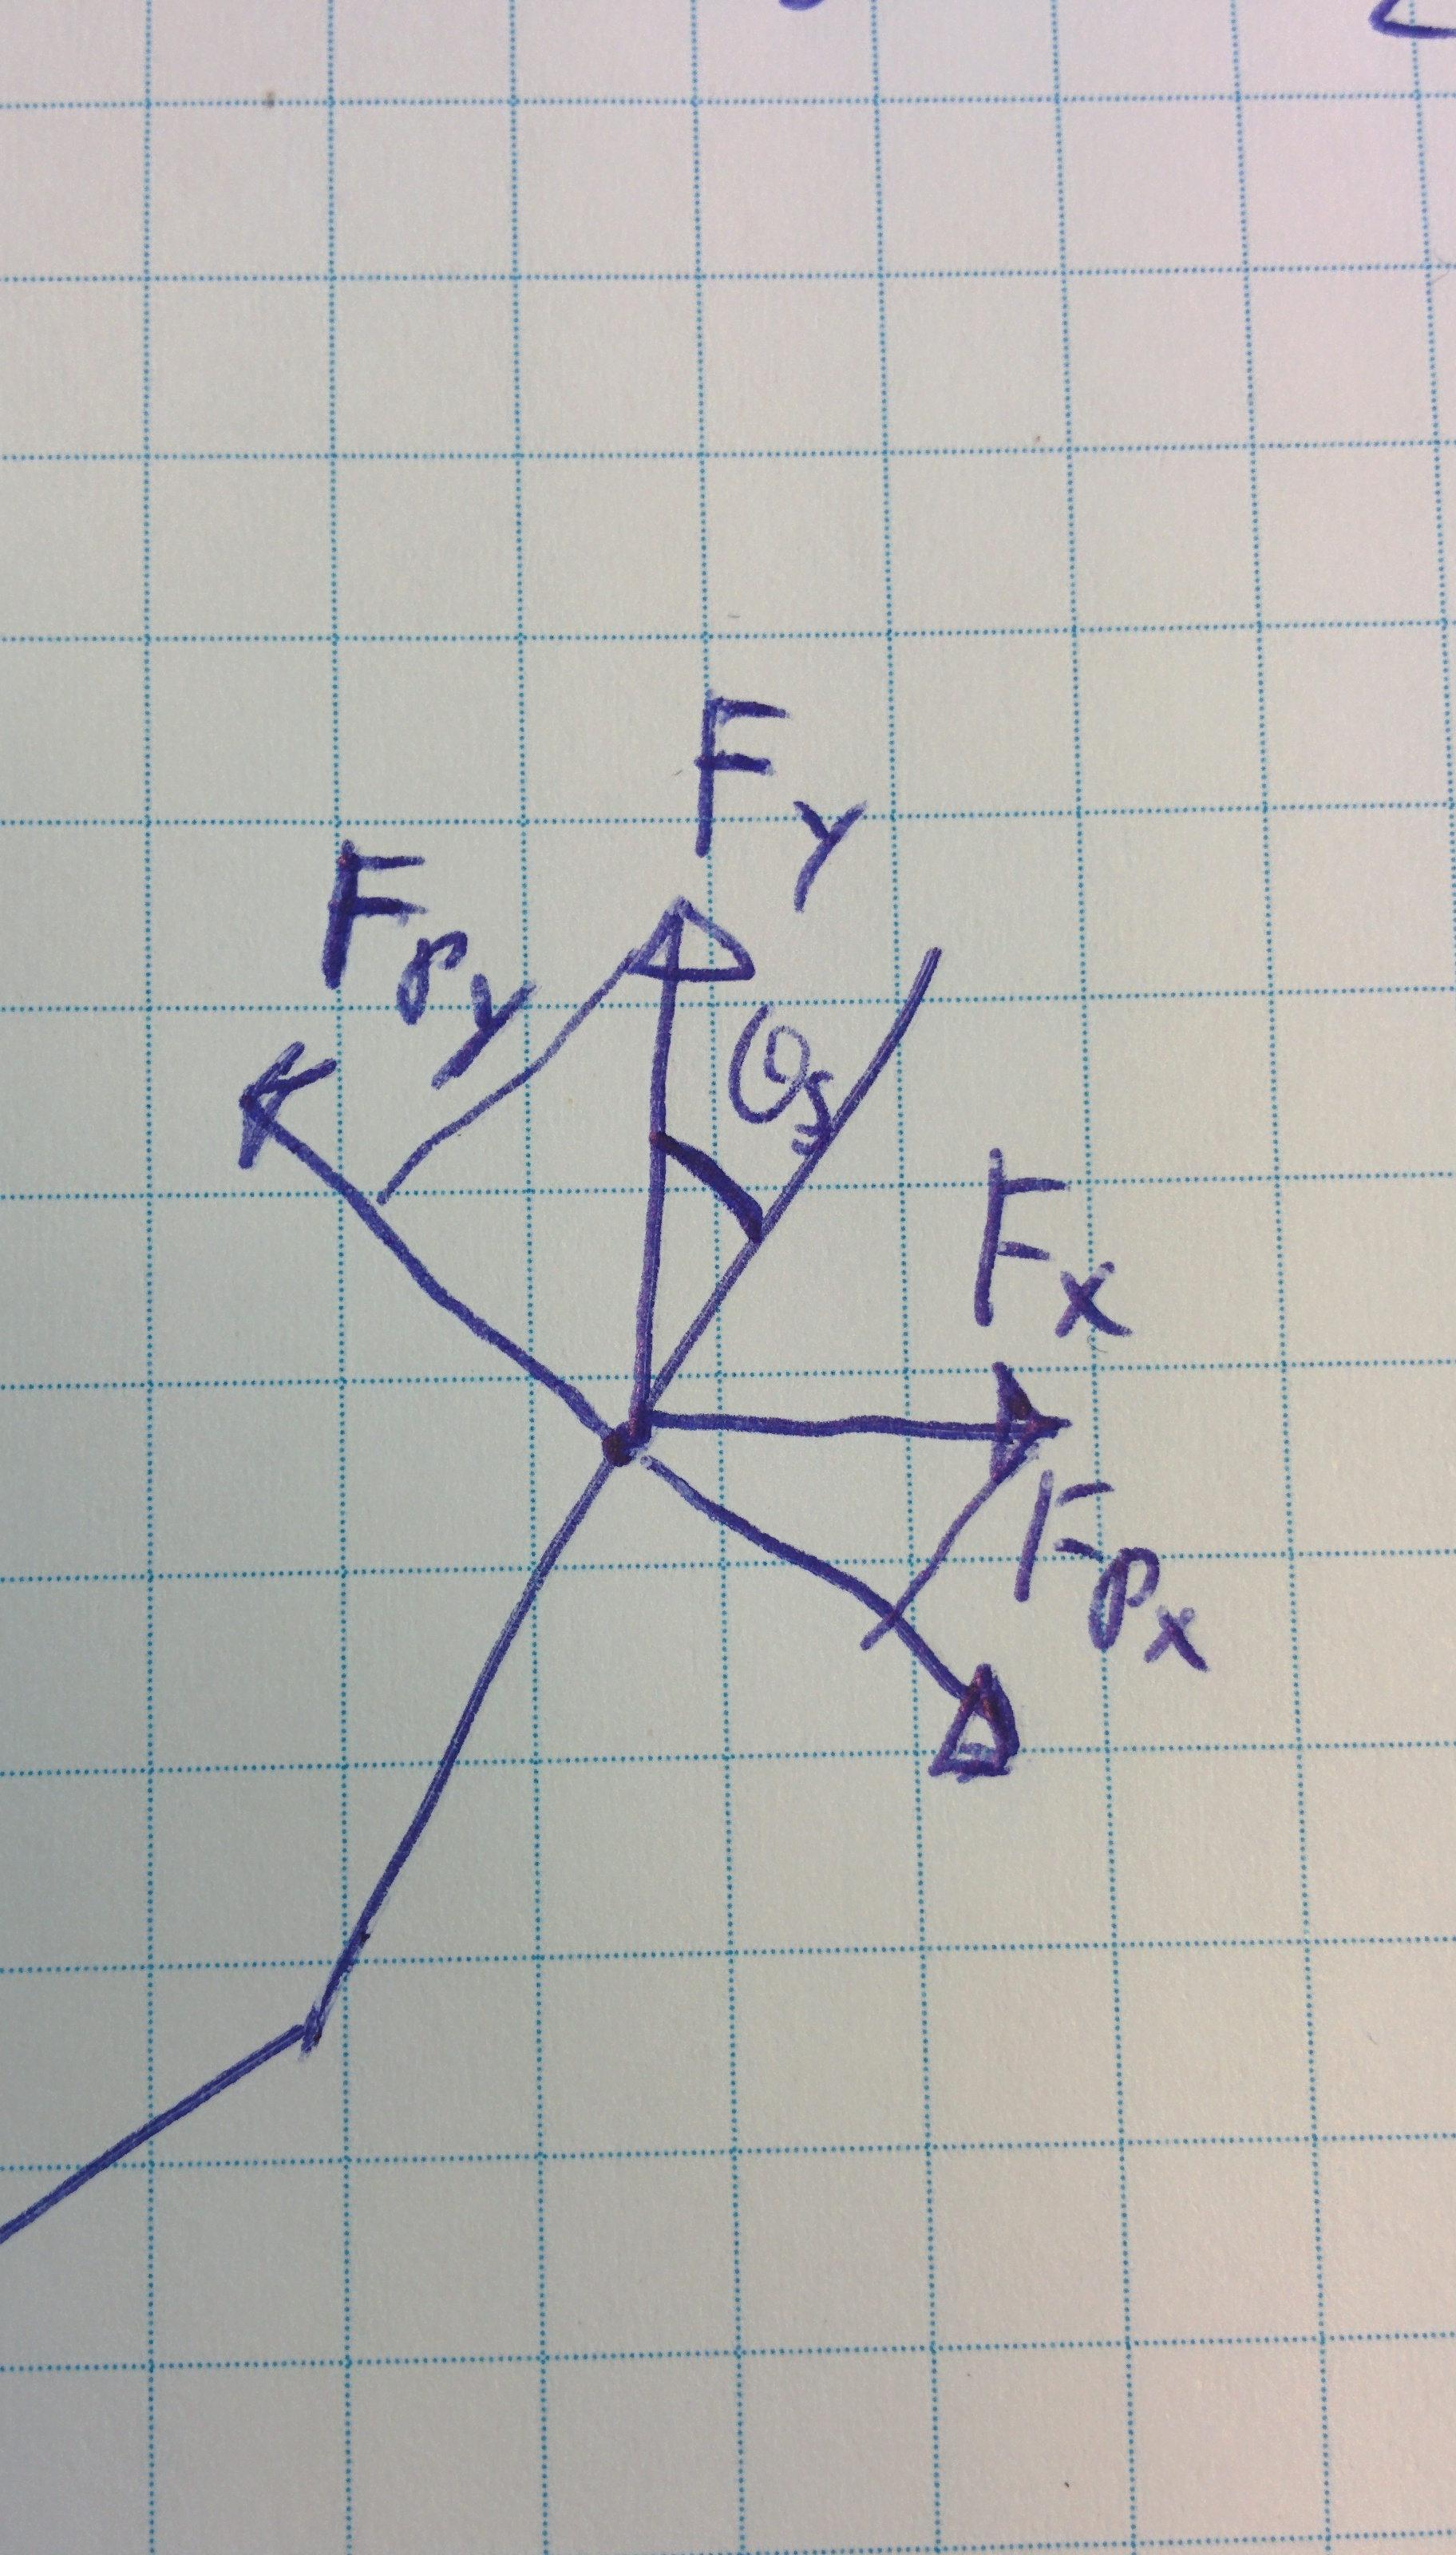
\includegraphics[width=0.25\textwidth]{ForcePerp}
%\caption{Diagram of the forces, $F_x$ and $F_y$, decomposed into perpendicular forces.}
%\label{fig:ForcePerp}
%\end{figure}

%\begin{subequations}\label{eq:perpFxFy}
%\begin{flalign}
%& F_{px}=F_x\cos(\theta_s) \\
%& F_{py}=F_y\sin(\theta_s)  \\
%& F_p = F_{px}+F_{py} 
%\end{flalign}
%\end{subequations}

The derivatives of the two geometric equations are inserted into \autoref{eq:transx} and \autoref{eq:transy} which are then inserted into \autoref{eq:rotaryforce} in \autoref{eq:JsLong}.
\begin{subequations}
\begin{flalign}
 J_s\ddot{\theta}_s &=\frac{l_s}{2}\left(\ddot{x}_sM_s\cos(\theta_s)+\left(\ddot{y}_s+g\right)M_s\sin(\theta_s)\right)-b_{as}\dot{\theta}_{as}  \\
 J_s\ddot{\theta}_s = \frac{l_s}{2}M_s \Big( &-l_a\ddot{\theta}_a\left(\cos(\theta_a)\cos(\theta_s)+\sin(\theta_a)\sin(\theta_s)\right) \notag \\
& +l_a\dot{\theta}_a^2\left(\sin(\theta_a)\cos(\theta_s)-\cos(\theta_a)\sin(\theta_s)\right) \notag \\
& -\frac{l_s}{2}\ddot{\theta}_s\left(\cos(\theta_s)\cos(\theta_s)+\sin(\theta_s)\sin(\theta_s)\right) \notag \\
& +\frac{l_s}{2}\dot{\theta}_s^2\left(\sin(\theta_s)\cos(\theta_s)-\cos(\theta_s)\sin(\theta_s)\right)  \notag \\
& +g\sin(\theta_s) \Big)-b_{as}\dot{\theta}_{as} \label{eq:JsLong}
\end{flalign}
\end{subequations}

Using the trigonometric properties in \autoref{eq:trigprop}, \autoref{eq:JsLong} is reduced to \autoref{eq:JsShort}.
\begin{subequations} \label{eq:trigprop}
\begin{flalign}
& \cos(\theta_a)\cos(\theta_s)\pm \sin(\theta_a)\sin(\theta_s)=\cos(\theta_a \mp \theta_s)  \\
& \sin(\theta_a)\cos(\theta_s)\pm \cos(\theta_a)\sin(\theta_s) = \sin(\theta_a \pm \theta_s) \\ 
& \cos(\theta_s)^2+\sin(\theta_s)^2=1 
\end{flalign}
\end{subequations}
\begin{flalign}
J_s\ddot{\theta}_s = \frac{l_s}{2}M_s \Big( &-l_a\ddot{\theta}_a \cos(\theta_a-\theta_s)+l_a\dot{\theta}_a^2 \sin(\theta_a-\theta_s) \notag \\
&-\frac{l_s}{2}\ddot{\theta}_s +g\sin(\theta_s) \Big)-b_{as}\dot{\theta}_{as} \label{eq:JsShort}
\end{flalign}

This is the nonlinear mathematical model for the system. This will be linearized in order to perform a Laplace transformation. The linearization is found in \autoref{sec:LinearStick}.

The linearized model is \autoref{eq:LinStick}.
\begin{flalign}
& J_s\ddot{\theta}_s=\frac{l_s}{2}M_s\left(-l_a\ddot{\theta}_a-\frac{l_s}{2}\ddot{\theta}_s+g\theta_s\right)-b_{as}\dot{\theta}_{as} \label{eq:LinStick}
\end{flalign}

Inserting the moment of inertia for a rotating stick, $J_s=\frac{1}{12}M_sl_s^2$, the linearized model becomes \eqref{eq:JsFinal} \cite{web:MInertia}.
\begin{subequations}
\begin{flalign}
& \frac{1}{12}M_sl_s^2\ddot{\theta}_s=\frac{l_s}{2}M_s\left(-l_a\ddot{\theta}_a-\frac{l_s}{2}\ddot{\theta}_s+g\theta_s\right)-b_{as}\dot{\theta}_{as}   \\
& \frac{1}{12}M_sl_s^2\ddot{\theta}_s+\frac{1}{4}M_sl_s^2\ddot{\theta}_s=\frac{l_s}{2}M_s\left(-l_a\ddot{\theta}_a+g\theta_s\right)-b_{as}\dot{\theta}_{as}   \\
& \frac{1}{3}M_sl_s^2\ddot{\theta}_s=\frac{l_s}{2}M_s\left(-l_a\ddot{\theta}_a+g\theta_s\right)-b_{as}\dot{\theta}_{as}  \label{eq:TauSmLin} \\
& \ddot{\theta}_s=\frac{3}{2l_s}\left(-l_a\ddot{\theta}_a+g\theta_s\right)-\frac{3b_{as}\left(\dot{\theta}_s-\dot{\theta}_a\right)}{M_sl_s^2} \label{eq:JsFinal}
\end{flalign}
\end{subequations}

The linearized model is now Laplace transformed in \autoref{eq:tfArmStick} in order to find the transfer function.
\begin{subequations}
\begin{flalign}
& s^2\Theta_s=\frac{3}{2l_s}\left(-s^2l_a\Theta_a +g\Theta_s\right)-s\frac{3b_{as}}{M_sl_s^2}\Theta_s+s\frac{3b_{as}}{M_sl_s^2}\Theta_a  \\
& \Theta_s\left(s^2+\frac{3b_{as}}{M_sl_s^2}s-\frac{3g}{2l_s}\right)=\Theta_a\left(-\frac{3l_a}{2l_s}s^2+\frac{3b_{as}}{M_sl_s^2}s\right)  \\
& \frac{\Theta_s}{\Theta_a}=\frac{-\frac{3l_a}{2l_s}s^2+\frac{3b_{as}}{M_sl_s^2}s}{s^2+\frac{3b_{as}}{M_sl_s^2}s-\frac{3g}{2l_s}} \label{eq:tfArmStick}
\end{flalign}
\end{subequations}

The system has a zero in 0 (two if the friction is considered negligible) which gives a 0 dB DC gain. This makes sense as the stick shouldn't move if the angle of the arm is constant. The poles show that the natural frequency of the system depends only on the gravity and length of the stick. This is similar to \autoref{eq:pendulum} for the frequency of a simple pendulum \cite{web:Pendulum}.
\begin{flalign}\label{eq:pendulum}
\omega_n=\sqrt{\frac{g}{L}}
\end{flalign}

A linearized model in the Laplace domain for the arm and the stick has been derived and the model for the motor and gears is now derived. The load torque generated by the arm and stick is significantly smaller than that of the gear system at the DC motor and is therefore assumed negligible.
